\documentclass[a4paper, 11pt, oneside]{book}
\usepackage{fancyhdr}
\pagestyle{fancy}
% i comandi seguenti impediscono la scrittura in maiuscolo
% dei nomi dei capitoli e dei paragrafi nelle intestazioni
\renewcommand{\chaptermark}[1]{\markboth{#1}{}}
\renewcommand{\sectionmark}[1]{\markright{\thesection\ #1}}
\fancyhf{} % rimuove l’attuale contenuto dell’intestazione
% e del pi\‘e di pagina
\fancyhead[LE,RO]{\bfseries\thepage}
\fancyhead[LO]{\bfseries\rightmark}
\fancyhead[RE]{\bfseries\leftmark}
\renewcommand{\headrulewidth}{0.5pt}
\renewcommand{\footrulewidth}{0pt}
\addtolength{\headheight}{0.5pt} % riserva spazio per la linea
\fancypagestyle{plain}{%
\fancyhead{} % ignora, nello stile plain, le intestazioni
\renewcommand{\headrulewidth}{0pt} % e la linea
}

\usepackage[italian]{babel}
\usepackage[utf8]{inputenc}
\usepackage{makeidx}
\usepackage{amsfonts}
\usepackage{amsmath}
\usepackage{amsthm}
\usepackage{amssymb}
\usepackage{graphicx}
\usepackage{verbatim}
\usepackage[symbol]{footmisc}
\usepackage[T1]{fontenc}
\usepackage{listings}
\usepackage[usenames,dvipsnames]{xcolor}
\usepackage{enumerate}

\usepackage{hyperref}

\definecolor{orange}{rgb}{1,0.5,0}

\tolerance=1
\emergencystretch=\maxdimen
\hyphenpenalty=10000
\hbadness=10000

\newcommand{\files}[1]{\texttt{#1}}


\newcommand{\zz}{\mathbb{Z}}
\newcommand{\nn}{\mathbb{N}}

\frenchspacing

\newenvironment{dimo}{\textbf{Dimostrazione.\ }}{\samepage
\begin{flushright}$\blacksquare$\end{flushright}}

\newtheorem{teo}{Teorema}[chapter]
\newtheorem{prop}[teo]{Proposizione}
\newtheorem{cor}[teo]{Corollario}
\newtheorem{lemma}[teo]{Lemma}


\theoremstyle{definition}
\newtheorem{defi}[teo]{Definizione}
\newtheorem{osse}[teo]{Osservazione}
\newtheorem*{exe}{Esercizio}
\newtheorem*{ese}{Esempio}
\newtheorem*{notabene}{Nota Bene}
\newtheorem*{nota}{Nota}

\theoremstyle{remark}
\newtheorem*{notazione}{Notazione}

% General command to set parameter(s).
\lstset{
 %belowcaptionskip=1\baselineskip,
 basicstyle=\footnotesize\ttfamily,
 keywordstyle=\bfseries\color{Purple},
 commentstyle=\itshape\color{ForestGreen},
 identifierstyle=\color{blue},
 stringstyle=\color{orange},
 showstringspaces=false,
 otherkeywords={simple, gates, parameters, simtime_t, simsignal_t, cMessage, channel},
 %breakindent = 20pt,
 breakautoindent = True,
 postbreak=\space,
 breaklines,
 tabsize = 2,
 language = C++,
 %frameround = tttt,
 frame = L %shadowbox
}
%\renewcommand{\lstlistingname}{}

\author{Fabio Biselli}
\title{Relazione di Progetto (bozza)}
\date{}

\begin{document}
\begin{titlepage}

\begin{center}
\Large UNIVERSIT\`A DEGLI STUDI DI BOLOGNA\\
Dipartimento di Informatica - Scienza e Ingegneria\\
\bigskip
\Large Corso di Laurea Magistrale in Informatica\\
\vspace{100pt}
\huge \textbf{Relazione di progetto: simulazione di un
ambiente virtuale distribuito}
\end{center}

\vspace{100pt}
\large
\begin{center}
\textbf{Dott. Fabio Biselli}
\end{center}
\normalsize
\bigskip
\begin{center}
Simulazione di Sistemi. Anno Accademico 2014/2015
\end{center}
\end{titlepage}

\tableofcontents

\chapter{Introduzione}
L'utilizzo di schede grafiche professionali ad elevate prestazioni offrono
oggi un ottimo \emph{frame-rate} per il rendering in tempo reale di complessi
scenari 3D. Le connessioni Internet veloci sono diventate disponibili un po'
in tutto il mondo ad un relativo basso costo.
Questi due fattori hanno contribuito allo sviluppo ed alla crescita di ambienti
virtuali distribuiti (Distribuited Virtual Environment Systems -- DVE).

Questi sistemi consentono ad una moltitudine di utenti, che utilizzano
client differenti, interconnessi mediante reti differenti (internet), di
interagire all'interno di un ambiente condiviso. Ogni utente è rappresentato
all'interno del DVE da un'entità chiamata \emph{avatar} controllata dall'utente
tramite il computer client.

I Sistemi DVE sono attualmente utilizzati in tante applicazioni, quali
l'addestramento civile e militare, il design collaborativo, alcune piattaforme
di e-learning ed il gioco multiplayer online (MMOGs).
Poichè i DVE supportano interazioni visuali tra molti avatar, occorre notificare
ogni client circa i cambiamenti posizionali degli avatar vicini.
Inoltre, essendo basati su piattaforme differenti ed essendoci parecchi fattori
che rendono i DVE inerentemente eterogenei, la definizione di una metodologia
generica per il design di sistemi DVE efficienti è un'attività complessa.
Alcuni aspetti che sono stati studiati a questo scopo sono:
\begin{itemize}
\item
\emph{Data Model:} descrive alcuni metodi per distribuire dati persistenti o
semipersistenti in un DVE.
\item
\emph{Communication Model:} analizza i metodi con cui gli avatar comunicano
tra di loro e come questo influenzi le performance del sistema.
\item
\emph{View Consistency:} mira ad assicurare che ogni avatar che condividono
un'area comune abbiano la medesima percezione degli oggetti presenti.
\item
\emph{Network Traffic Reduction:} mantenere un basso numero di messaggi
permette ai sistemi DVE di scalare in modo efficiente con il numero
degli avatar connessi.
\item
\emph{Partitioning Problem:} individuare un modo efficiente per assegnare
a più server la gestione degli avatar consente di migliorare le performance
generali del DVE.
\end{itemize}

L'articolo
\cite{IDVE}
studiato per il progetto, su cui si basa
principalmente il modello proposto,
studia il problema della partizione. Gli autori descrivono un modello di DVE
(sintetizzato nella sezione \ref{modello_orig}) sperimentando mediante
la simulazione la correlazione tra la \emph{funzione di qualità}
\footnote{La funzione di qualità $C_P$ è definita come:
$C_P = W_1 \cdot C_P^W + W_2 \cdot C_P^L$,  dove $W_1 + W_2 = 1$. $W_1$ e $W_2$
sono due coefficienti relativi al peso del lavoro di computazione e di
comunicazione rispettivamente.} proposta nella
letteratura e le prestazioni del sistema (DVE System). Poiché i risultati
mostrano assenza di correlazione ed un comportamento non-lineare in relazione
al numero degli avatar gli autori propongono un nuovo metodo di partizione.
Con questo metodo, basato sul bilanciamento del carico dei server, mostrano
che è possibile mantenere il carico al di sotto della soglia in cui
le prestazioni medie del DVE degradano velocemente, questo a prescindere dal
numero di avatar, dalla loro distribuzione iniziale e dal pattern di movimento.

Nel presente progetto si vuole invece analizzare un nuovo modello, derivato
da quello proposto nell'articolo ma con alcune modfiche, per studiarne il
comportamento della comunicazione rispetto al traffico della rete.
Grazie a risultati evidenziati nel suddetto articolo è possibile trascurare
il problema del carico dei server assumendo che, grazie all'algoritmo di
partizione, il \emph{delay} delle comuncazioni sia influenzato in modo
trascurabile. Nonostante questo si è comunque deciso di implementare un
semplice algoritmo di partizionamento per il modello, in modo da poter valutare
il traffico dati relativo all'aggiornamento sia dei server che dei client
del sistema.

Il Capitolo \ref{setup} introduce la caratterizzazione ed il setup dei
modelli. Si propone una sintesi del modello dell'articolo, al fine di poter
meglio confrontare la seguente e più ampia descrizione del modello proposto.

Nel Capitolo \ref{impl} vengono descritti i principali dettagli implementativi
del modello, con più attenzione sui file di descrizione (\texttt{NED}),
la definizione di messaggi (\texttt{.msg}) e file di configurazione
(\texttt{.ini}) del framework \texttt{OMNeT++} rispetto alle semplici classi
\texttt{C++}.

Il Capitolo \ref{analisi} è dedicato all'esposizione ed all'analisi dei
risultati ottenuti mediante la simulazione.

Infine il Capitolo \ref{conclusioni} presenta alcune conclusioni ed alcuni
possibili sviluppi futuri.


\chapter{Caratterizzazione e Setup}\label{setup}
\section{Sintesi del sistema originale}\label{modello_orig}
Il sistema introdotto nell'articolo ed illustrato in figura \ref{fig1}
è così composto:
\begin{itemize}
\item
$3$ server, di cui uno contrassegnato come principale;
\item
$180$ client che controllano un avatar nel mondo virtuale;
\item
una rete che connette i client ai server (che sono tra loro interconnessi);
\item
un ambiente virtuale (Virtual Environment);
\item
un metodo ed un file di partizionamento che il server principale utilizza per
suddividere il carico tra i server.
\end{itemize}

Il sistema di partizionamento per l'assegnamento dei client ad un server è
basato sul concetto di Area d'Interesse di un avatar (AoI). Ovvero se due
avatar condividono la medesima AoI dovrebbero essere gestiti dal medesimo
server.

All'inizio della simulazione gli avatar (client) sono distribuiti nell'ambiente
virtuale in modo uniforme.

La simulazione consiste nel far compiere ad ogni avatar $100$ movimenti, uno
ogni $2$ secondi. Quando l'avatar compie un movimento invia un messaggio di
ACK al server associato che lo propaga ai client nella relativa AoI.
I client che ricevono l'ACK rispediscono il messaggio al server che notifica
l'ACK ricevuto al client che ha effettuato lo spostamento. In questo modo è
possibile calcolare i tempi di risposta del sistema.
Alla fine della simulazione ogni client può calcolare il tempo medio di
risposta del sistema.

\begin{figure}
\label{fig1}
\begin{center}
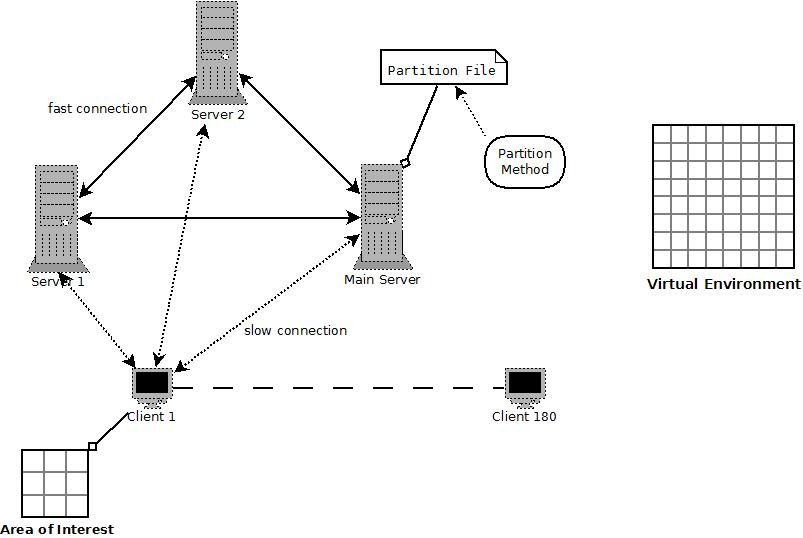
\includegraphics[scale=0.50]{schema.jpeg}
\end{center}
\caption{Schema proposto nell'articolo di riferimento.}
\end{figure}


\section{Definizione di un nuovo modello}

In questa sezione sono descritte le principali caratteristiche per
l'implementazione del nuovo modello proposto. Si può schematizzare il
sistema descritto in figura \ref{fig2} nel seguente modo:
\begin{itemize}
\item
$1$ Main Server che si occupa del login dei client e della gestione
dell'ambiente simulato;
\item
$k \in \{1, \ldots, 9\}$ server di partizione che si occupano di gestire i
messaggi tra client ed aggiornare il Main Server;
\item
$n$ client che controllano un distinto avatar nel mondo virtuale;
\item
una rete WAN simulata che connette i client ai server;
\item
una rete LAN simulata che connette i server con una struttura ad anello
unidirezionale;
\item
un ambiente virtuale (\texttt{VirtualEnvironment});
\item
un metodo di partizionamento statico, dipendente dal numero di server di
partizione, che il Main Server utilizza per suddividere il carico.
\end{itemize}

\subsection{Impostazioni iniziali}
Nell'articolo vengono descritte due diverse simulazioni con numeri di server
e client fissi. L'implementazione di questa simulazione, basata su OMNet++,
prevede un parametro per i server ed uno per i client in modo tale che l'utente
possa specificarne il numero (file \texttt{.ini}).

Si suppone che inizialmente gli avatar siano distribuiti nell'ambiente virtuale
con una distribuzione casuale uniforme e che non siano già presenti nella
suddetta ma debbano effettuare il login sul server principale con un ritardo
variabile (distribuzione esponenziale) dall'inizio della simulazione.

\subsection{Ambiente virtuale}
L'ambiente virtuale è una semplicissima struttura: un array
bidimensionale di mappe di Avatar
(\texttt{$\langle$id, VirtualAvatar$\rangle$}).
Questa ``simula'' un'area in cui gli avatar possono muoversi liberamente e
senza collisioni. Per l'implementazione si utilizzano due classi distinte
per gli avatar: \texttt{Avatar} utilizzata dai client e
\texttt{VirtualAvatar} utilizzata dal Main Server.

\subsection{Avatar e VirtualAvatar}
\texttt{Avatar} è una semplice classe sfruttata dal client per rappresentare
la posizione attuale all'interno dell'ambiente virtuale.
\texttt{VirtualAvatar} è la classe che rappresenta l'avatar all'interno
dell'ambiente virtuale gestito dal Main Server. Entrambe le classi sono
ausiliarie alla gestione dei movimenti lato client e lato server,
rispettivamente.

%% Ha quattro campi: oltre agli interi che
%% rappresentano id e coordinate utilizza un puntatore all'ambiente virtuale.

\subsection{Gestione dell'ambiente e dei movimenti}
L'ambiente virtuale viene modificato dal Main Server tramite messaggi da parte
dei server di Partizione che, grazie alle notifiche dei
movimenti da parte dei client, rimuovono l'avatar dalla vecchia cella
e lo assegnano a quella di destinazione.

A questo punto vengono aggiornati i client coinvolti, ovvero nel momento
in cui un avatar si sposta, il Server di Partizione:
\begin{enumerate}
\item
notifica ai vicini che l'avatar lascia la casella;
\item
notifica al Main Server lo spostamento, il quale calcola ed invia la nuova
AoI;
\item
attende l'arrivo della nuova AoI ed inoltra la notifica ai nuovi vicini ed al
client stesso.
\end{enumerate}

I movimenti degli avatar, che avverranno ogni due secondi, avranno come
destinazione una delle caselle adiacenti (compresa la casella di partenza,
in tal caso nessun messaggio sarà inoltrato nel sistema). Tuttavia,
come evento eccezionale (con una bassa probabilità), ogni avatar potrà
effettuare un ``Jump'' ad una casella casuale all'interno del mondo.

\subsection{Connessioni}
I server sono interconnessi, mediante ``channel'' con un basso delay
per simulare una connessione intranet (LAN). Mentre per le connessioni
client-server è stato introdotto un modulo (\texttt{WAN}) apposito per simulare
una latenza più alta e variabile, che imiti il comportamento della rete
internet.

\subsection{Metodo di partizionamento}
Il metodo di partizionamento, poiché non è oggetto dello studio, è stato
implementato in modo semplificato. Ad ogni server viene assegnata una porzione
del mondo in modo lineare. Questo introduce un vincolo sul un numero massimo di
server che l'utente può specificare all'avvio.

\begin{figure}
\begin{center}
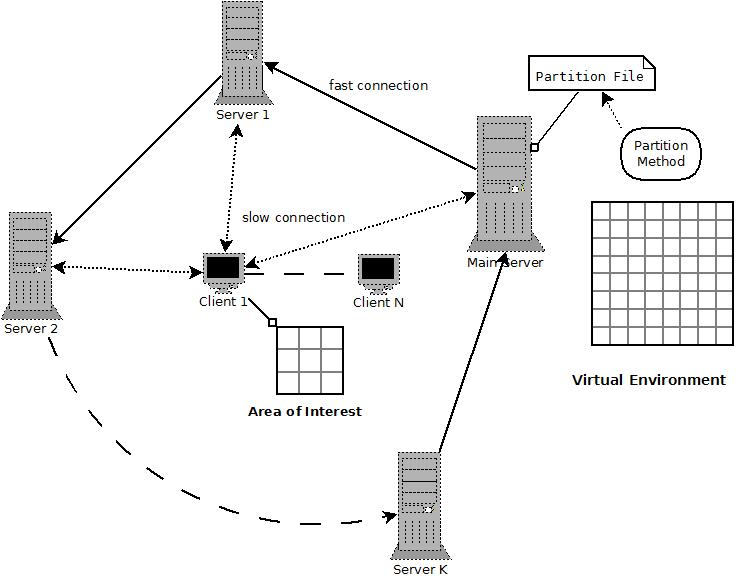
\includegraphics[scale=0.50]{schemaRing.jpeg}
\end{center}
\caption{Schema proposto per l'implementazione.}
\label{fig2}
\end{figure}

\subsection{Simulazione di eventi}
Il sistema simula l'interazione da parte di utenti (che possono essere giocatori
di un gioco distribuito o utenti di un simulatore per l'addestramento militare
o civile) con un ambiente virtuale, ogni utente può interagire con il mondo
virtuale mediante un client (\files{DVEClient}). Il client è connesso tramite
la rete WAN (internet) al sottosistema server che gestisce il gioco o la
sessione di addestramento, ogni qual volta l'utente effettua un movimento che
induca un cambio di stato del mondo virtuale, il client invia un messaggio di
movimento (\files{MoveMsg}) al server.

A differenza del modello proposto nell'articolo, in cui tutti gli avatar vengono
attivati all'inizio della simulazione, ogni avatar entra nel mondo virtuale
dopo un tempo variabile. A questo scopo è stato introdotto un secondo tipo
di evento: il login. All'avvio della simulazione l'ambiente virtuale
risulta vuoto, si popola man mano che i client effettuano il login.
Dopo il login ogni avatar esegue un movimento ogni due secondi come previsto
dal modello originale.

\chapter{Implementazione del modello}\label{impl}
L'implementazione del modello proposto è stata realizzata mediante il framework
\texttt{OMNeT++}. \texttt{OMNeT++} è una libreria estensibile e modulare
basata su \texttt{C++} creata principalmente per la simulazione di reti.
La sua estensibilità ed il vantaggio di essere open-source ha permesso lo
sviluppo di molti moduli da parte della comunità. Nel presente progetto
è stato utilizzato per alcune funzionalità il pacchetto \texttt{queueinglib}.

Per la realizzazione del modello è stato utilizzato il linguaggio di
scripting di \texttt{OMNeT++} per la definizione delle entità quali i client,
i Server di Partizione, il Main Server e i canali di comunicazione
(\texttt{NED} files), la definzione dei messaggi (\texttt{msg} files) e
la struttura generale della rete. La logica sottostante è stata invece
interamente scritta in \texttt{C++}. La configurazione della simulazione
è resa editabile mediante il file di configurazione \texttt{omnetpp.ini}.

La parte lato client è composta dalle classi \texttt{Avatar}, \texttt{DVEClient}
e dai moduli \texttt{DVEClient.ned} e \texttt{Source} (da \texttt{queueinglib}).
Per il lato server sono state implentate le seguenti classi: \texttt{DVEServer},
\texttt{MainServer}, \texttt{VirtualEnvironment} e \texttt{VirtualAvatar}, ed
i moduli \texttt{DVEServer.ned} e \texttt{MainServer.ned}.
Per quanto riguarda la comunicazione è stata implementata la classe
\texttt{WAN}, il modulo \texttt{WAN.ned} ed i messaggi (con le relative classi
\texttt{C++} autogenerate) \texttt{ACKMsg}, \texttt{LoginMsg}, \texttt{MoveMsg},
\texttt{ServerUpdateMsg} e \texttt{UpdateAoIMsg}. La definizione della rete,
ovvero del modello, specificata nel modulo \texttt{DVESystem.ned}.
Per un totale di $12$ classi \texttt{C++}, $5$ moduli \texttt{NED} e
$5$ definizioni di messaggi.

\section{Client}
Il client, come suggerisce il nome, rappresenta il cliente di un servizio. Sia
questo una recluta militare o civile, uno studente o un giocatore di un MMO, si
aspetta di ricevere un servizio che sia almeno accettabile.
\`E noto che la natura della rete internet, ambiente in cui principalmente
lavorano i DVE, è di tipo ``best effort'', ovvero non vi sono garanzie riguardo
alla comunicazione dei messaggi. \`E quindi ragionevole domandarsi e cercare
di capire con la simulazione quanto un DVE sia affidabile dal punto di vista
dei client. Le classi ed i moduli introdotti in questa sezione hanno questa
finalità.

\subsection{\texttt{Avatar}}
La classe \files{Avatar} rappresenta l'utente nell'ambiente virtuale, mantiene
i dati relativi alla posizione attuale ed ai vicini, ovvero altri utenti nella
medesima Area di Interesse.
Ha quattro campi: un \files{ID} che si riferisce al client (\texttt{getIndex()}
in \texttt{simpleModule} di \texttt{OMNet++}), due interi che rappresentano le
coordinate
all'interno dell'ambiente virtuale (\texttt{x, y}) e un vettore di interi che
rappresentano (mediante id univoco) gli altri avatar nella propria Area di
Interesse.

\subsection{\texttt{Source}}
Il modulo \texttt{Source} è l'unico costrutto della libreria
\texttt{queueinglib} utilizzato nel modello. Fondamentalmente simula le azioni
dell'utente nell'utilizzo del client, esso infatti genera automaticamente e
ad intervalli regolari un numero fissato di \texttt{jobs} che invia al modulo
\texttt{DVEClient}, come descritto nel prossimo paragrafo tutta la logica delle
azioni è definita nel client. Per ogni utente simulato viene generato un
modulo \texttt{Source} collegato al client mediante canale unidirezionale
privo di latenza.

\subsection{\texttt{DVEClient}}
Il client vero e proprio è definito dal modulo \texttt{DVEClient} e dalla
relativa classe \texttt{C++} che ne definisce il comportamento.
\subsubsection{Modulo \files{NED}}
Il modulo è connesso, oltre che al suddetto \texttt{Source} in solo ingresso,
ad un modulo che simula la rete (\texttt{WAN}) mediante un canale bidirezionale.
Il canale è privo di latenza in quanto, come descritto nella relativa sezione,
il nodo che simula internet si occupa di emularne il comportamento.
Oltre ai \texttt{gates} qui vi sono registrati i parametri per le statistiche
di interesse del client:
\begin{itemize}
\item \textbf{Risposta del sistema}: calcola il tempo simulato di risposta
del sistema, ovvero ad ogni movimento del client misura il tempo impiegato
per notificare tutti i client (vicini nuovi e vecchi) e server coinvolti.
\item \textbf{Movimenti persi}: tiene conto dei movimenti persi di ogni client.
Quando un nuovo \texttt{job} arriva al client per effettuare un movimento, se
non è ancora arrivata la notifica (ACK) del movimento precedente non è possibile
effettuare il nuovo movimento (effetto \emph{lag}).
\item \textbf{Movimenti nulli}: conta i movimenti non effettuati ``volutamente''
dall'utente.
\item \textbf{Movimenti}: conta i movimenti effettuati con successo.
\item \textbf{Presence Factor}: conta la ``numerosità'' della AoI, ovvero
il numero di altri avatar nella medesima zona..
\end{itemize}
Come si può notare nel listato \ref{clientNED} ogni voce di cui sopra è
realizzata mediante il meccanismo del \emph{signaling}, utilizzando un
\texttt{@signal} che rileva i segnali emessi dai relativi eventi
ed una \texttt{@statistic} che ne registra i valori in un apposto vettore.
Questi dati saranno quindi utilizzati per analizzare la simulazione.

\begin{lstlisting}[caption = {Il Modulo DVEClient.},
                   label = {clientNED}]
simple DVEClient
{
  parameters:
    @signal[sysResponse](type="simtime_t");
    @statistic[dveResponse](...);
    @signal[moveLost](type="int");
    @statistic[clientMovesLost](...);
    @signal[noMove](type="int");
    @statistic[clientNoMoves](...);
    @signal[move](type="int");
    @statistic[clientMoves](...);
    @signal[presenceFactor](type="unsigned int");
    @statistic[clientPresenceFactor](...);
  gates:
    inout wanIO;
    input fromSource;
}
\end{lstlisting}

\subsubsection{Classe \files{DVEClient}}
Per quanto riguarda la realizzazione della logica, che consente al client di
comunicare con il Sistema e di emettere i segnali degli eventi da registrare,
è stata realizzata una classe \texttt{C++} derivata da \texttt{cSimpleModule}
della libreria \texttt{omnetpp.h}:
\begin{lstlisting}
#include <omnetpp.h>

class DVEClient : public cSimpleModule {
private:
  ...
\end{lstlisting}
Questo pattern è stato utilizzato per ogni modulo \texttt{NED} realizzato e
verrà pertanto omesso da qui in avanti.
\begin{lstlisting}
  // The game avatar.
  Avatar* avatar;
  // The current game server id that the client refers to.
  int serverID;
  // Flag to login the client.
  bool logged;
  // Flag: is the AoI updated?
  bool ready;
  // Flag: has the client lost a move?
  bool frozen;
\end{lstlisting}
Per la gestione dello stato interno all'ambiente virtuale la classe include un
\files{Avatar}, un ID univoco ed alcuni flag atti ad individuare se il login
è già avvenuto, se il sistema ha aggiornato correttamente l'ultimo movimento
del client e se l'ultimo tentativo di movimento non è andato a buon fine.
\begin{lstlisting}
  // Statistics.
  simtime_t timeRequest;
  simsignal_t systemResponseSignal;
  int ackReceived;
  simsignal_t moveLostSignal;
  int movesLoss;
  simsignal_t noMoveSignal;
  int nomoves;
  simsignal_t moveSignal;
  int moves;
  simsignal_t presenceFactorSignal;
  unsigned int presenceFactor;
\end{lstlisting}
Per la gestione delle statistiche la classe include una variabile per ogni
statistica registrata nel modulo ed il segnale rispettivo.
\begin{lstlisting}
  void makeMove();
  void handleLoginMessage(cMessage *msg);
  void handleMoveMessage(cMessage *msg);
  void handleUpdateMessage(cMessage *msg);
  void handleUpdateAoIMessage(cMessage *msg);
  void handleACKMessage(cMessage *msg);
  void computeCoordinate(int src, int &dest);
\end{lstlisting}
I metodi della classe definiscono la logica ed il comportamento del client
in base agli eventi. Quando dal modulo \files{Source} arriva un messaggio,
se il client non è ``loggato'' (\files{logged == false}) vene inviata una
richiesta di login, altrimenti il metodo \texttt{makeMove()} genera un movimento
ed invia il messaggio al server. Ogni volta che dal server arrivano messaggi,
il metodo \files{handleMessage} (overloaded) invoca il metodo appropriato
come segue:
\begin{lstlisting}
void
DVEClient::handleMessage(cMessage *msg)
{
  LoginMsg* l_msg = dynamic_cast<LoginMsg*>(msg);
  if (l_msg != 0)
  {
    handleLoginMessage(msg);
    return;
  }
  MoveMsg* m_msg = dynamic_cast<MoveMsg*>(msg);
  if (m_msg != 0)
  {
    handleMoveMessage(msg);
    return;
  }
...
\end{lstlisting}
Analogamente alla definizione delle classi, questo pattern è utilizzato per ogni
altro modulo, verrà pertanto omesso nelle definizioni a seguire.
\subsubsection{Inizializzazione}
All'avvio della simulazione \texttt{OMNeT++} inizializza ogni modulo chiamando
il medoto \texttt{initialize()}, questo metodo risulta particolarmente
importante in quanto registra i segnali per le statistiche:
\begin{lstlisting}
  // Assuming the Avatar lives in a 9x9 world, and the
  // staring distribution among world cells is uniform.
  avatar = new Avatar(getIndex(), intuniform(0, 8), intuniform(0, 8));
  logged = false;
  ready = false;
...
  ackReceived = 0;
  WATCH(ackReceived);
  systemResponseSignal = registerSignal("sysResponse");
  presenceFactor = avatar->GetAoISize();
  WATCH(presenceFactor);
  presenceFactorSignal = registerSignal("presenceFactor");
\end{lstlisting}
Dopo aver inizializzato l'avatar ed altre proprietà, inizializza le statistiche,
le registra alla simulazione mediante la primitia \texttt{WATCH} e quindi
registra i vari segnali che verranno identificati da una stringa (identica
alla relativa variabile del modulo \texttt{NED}). A questo punto il client è
pronto per registrare gli eventi e le statistiche della simulazione.

\subsubsection{Movimento}
Come accennato, il movimento è l'unica azione che il client può compiere
(oltre al login iniziale). Per fare ciò, il suo stato deve essere
\texttt{logged} e \texttt{ready}, se questo avviene quando riceve un messaggio
da \texttt{Source} può invocare il metodo \texttt{makemove()}.
\begin{lstlisting}
  moves++;
  emit(moveSignal, moves);
...
  avatar->move(x, y);
  send(move, "wanIO,o");
  timeRequest = simTime();
\end{lstlisting}
Una volta calcolate le nuove coordinate, se non sono identiche a quelle
attuali, vengono aggiornate il numero di mosse, lo stato dell'avatar ed il
tempo simulato di invio della richiesta
(\texttt{timeRequest}), che sarà utile per calcolare il
tempo di risposta del sistema. Viene inoltre spedito un messaggio di movimento
(\texttt{move}) al server tramite la wan simulata.

\subsubsection{Risposta del sistema}
Una volta che il client ``decide'' di effettuare un movimento e quindi invia
una notifica al sistema, si mette in stato di attesa impostando il flag
\texttt{ready} a \texttt{false}. Il client non effettuerà più movimenti finchè
non riceverà la notifica da parte del sistema che il suo movimento è andato a
buon fine con conseguente aggiornamento dello stato dell'avatar (AoI).
\begin{lstlisting}
void
DVEClient::handleACKMessage(cMessage *msg)
{
...
  ready = true;
  ackReceived++;
  frozen = false;
  simtime_t response = simTime() - timeRequest;
  emit(systemResponseSignal, response);
  // Movement complete: update presence factor.
  presenceFactor = avatar->GetAoISize();
  emit(presenceFactorSignal, presenceFactor);
\end{lstlisting}
Quando arriva la notifica da parte del server tramite un messaggio di ACK
vengono aggiornati i flag di stato, viene calcolato il tempo di risposta
del sistema e viene quindi registrato emettendo tramite la primitiva
\texttt{emit} nel relativo vettore di statistiche. La medesima cosa avviene
per il \emph{Presence Factor}.

\section{Server}
La struttura lato server è il vero e proprio centro di calcolo del DVE, in
ogni campo di applicazione, dall'addestramento al gioco online, l'ambiente
virtuale viene gestito dal server, o meglio dai server.
L'articolo
\cite{IDVE}
definisce la struttura lato server come un ``numero di
server interconnessi''. Nel modello proposto si definisce un'archiettura più
specifica, i server sono infatti interconnessi tramite un anello circolare
unidirezionale.

I moduli implementati sono di due tipi: il Main Server che si occupa di gestire
l'ambiente virtuale e la partizione ed i Server di Partizione che si occupano
di gestire le comunicazioni con i client in base al partizionamento.

L'utente può specificare il numero di server di partizione
utilizzando il file di configurazione, vengono quindi creati tanti moduli
\texttt{DVEServer} quanti richiesti (da $1$ a $9$ per semplicità
indotta dal sistema statico di partizionamento).


\subsection{Main Server}
Il server principale è composto da un modulo \texttt{NED} con la relativa
implementazione \texttt{C++} nella quale sono inclusi una struttura dati per
la partizione del carico e l'ambiente virtuale in cui gli avatar virtuali
compiono i loro movimenti. Per l'implementazione dell'ambiente virtuale è stato
sfruttato un Design Pattern noto nell'industria videoludica
\cite{GamePattern}
come \emph{Spatial Pattern}.

\subsubsection{Modulo \texttt{NED}}
Il modulo è connesso alla LAN in sola uscita (anello unidirezionale) al primo
dei server (in ordine di id) ed in sola entrata all'ultimo. Un ulteriore
collegamento (bidirezionale) viene utilizzato per collegare direttamente
il server principale ai client, questo consente lo scambio di messaggi per
il login, quando ancora i client non sono stati assegnato ad un server di
partizione.
\begin{lstlisting}
simple MainServer
{
  parameters:
    int numOfServer;
    int numOfClient;
    @display("i=device/server2");
  gates:
    input lanIn;
    output lanOut;
    inout wanIO;
}
\end{lstlisting}

\subsubsection{Classe \texttt{MainServer}}
Analogamente a quanto visto per l'implementazione della classe client, la
class \texttt{MainServer} contiene una serie di attributi e metodi per
la gestione dell'ambiente virtuale ed i meccanismi di comunicazione con
il resto del sistema.
\begin{lstlisting}
  // The number of partition servers.
  int PARTSERVERS;
  // The maximum movements until apply a new server partition.
  int MOVESMAX;
  // The collection of clients logged in.
  std::map<int, VirtualAvatar*> connectedAvatars_;
  // The set of acknowledgments the server is waiting for.
  std::map<int, Acknowledgment*> ack_registry_;
  // The virtual environment.
  VirtualEnvironment* ve_;
  // An array of indexes representing the ve partition among servers.
  part_indexes* partition_;
  // Number of avatar movements since last server partition.
  int moves_n;
\end{lstlisting}
I commenti al codice di cui sopra sono autoesplicativi, occorre però evidenziare
un concetto finora non menzionato: come in \cite{IDVE} in un dato momento
della simulazione (in questo caso dopo un numero di movimenti totali che
dipendono dal numero di client previsti) avviene una ridistribuzione delle
partizioni. I parametri \texttt{MOVESMAX} e \texttt{moves\_n} hanno questo
scopo.

\subsubsection{Movimento}
Quando un messaggio di movimento arriva al Server Principale, innazitutto
questo si occupa di notificare la nuova AoI al client:
\begin{lstlisting}
  int* newAoi = NULL;
  unsigned int newAoiSize;
  ve_->GetAvatarAndSizeAt(x, y, &newAoi, newAoiSize);
  UpdateAoIMsg* update = new UpdateAoIMsg();
  update->setClientMoved(clientID);
  update->setX(x);
  update->setY(y);
  update->setAoiArraySize(newAoiSize);
  for (unsigned int index = 0; index < newAoiSize; index++)
  {
    update->setAoi(index, newAoi[index]);
  }
  update->setIsNeighborNotification(false);
  send(update, "lanOut");
\end{lstlisting}
Quindi aggiorna il mondo virtuale (il suo stato interno):
\begin{lstlisting}
    // Updates VA and VE.
    VirtualAvatar* avatar = connectedAvatars_[clientID];
    avatar->move(x, y);
\end{lstlisting}
Infine gestisce gli acknowledges, se non ci sono vicini nè nella vecchia AoI
nè in quella nuova notifica l'ACK al client, altrimenti genera un nuovo
\texttt{Acknowledgment} che si occupa di memorizzare gli ACK da parte dei
vicini. Quando il numero degli ACK ricevuto per il movimento è pari alla somma
delle due AoI viene generato ed inviato l'ACK per il client che potrà calcolare
così il tempo di risposta del sistema.

\subsection{Server di Partizione}
Il Server di Partizione è in realtà il server che si occupa di gestire le
comunicazioni tra i client ed il server principale. Il suo nome deriva
dall'approccio utilizzato per ridurre ed ottimizzare il tempo di risposta della
rete e del sistema.

\subsubsection{Modulo \texttt{NED}}
Il modulo è connesso alla LAN in sola uscita (anello unidirezionale) al
successore dei server (in ordine di id) o al Main Server se il server in
questione è quello con id più alto. \`E connesso in sola entrata al
predecessore dell'annello o al Main Server se è quello con id più basso. Un ulteriore
collegamento (bidirezionale) viene utilizzato per collegare direttamente
il server ai client, ovvero alla rete Internet (\texttt{WAN}).
\begin{lstlisting}
simple DVEServer
{
  @display("i=device/server");
  gates:
    input lanIn;
    output lanOut;
    inout wanIO;
}
\end{lstlisting}

\subsubsection{Classe \texttt{DVEServer}}
La classe \texttt{DVEServer} contiene tutta la logica relativa alla propagazione
dei messaggi all'interno del sistema. Questa permette ad un client di inviare
il movimento al server centrale, permette la propagazione degli ACK e dei
messaggi di aggiornamento delle AoI o delle partizioni.
Grazie alla definizione delle cinque differenti tipologie di messaggi, i server
riescono a consegnare sempre all'entità destinataria evitando
possibili cicli infiniti all'interno dell'anello LAN.

\section{Reti e comunicazione}
Quanto descritto fino ad ora rappresenta la struttura del sistema simulato,
tuttavia per poter far funzionare il tutto ed emulare un sistema distribuito
reale occorre simulare anche i canali e la rete di comunicazione.

Per quanto riguarda la LAN, ipotizzando una struttura creata appositamente
per il DVE, si è optato per canali con una latenza fissa molto bassa,
praticamente irrilevante. Mentre per simulare la rete Internet è stato creato
un modulo apposito: \texttt{WAN}.
\begin{lstlisting}
channel LAN extends ned.DelayChannel
{
  delay = 1ms;
}
\end{lstlisting}

\subsubsection{Modulo \texttt{NED}}
Il modulo è sostanzialmente un router per i messaggi, ha semplicemente tre
canali bidirezionali collegati ai client, ai server di partizione ed al server
principale.
\subsubsection{Classe \texttt{WAN}}
Analogamente alle altre classi, implementa la logica per la comunicazione.
L'unica differenza fondamentale che la caratterizza è l'utilizzo della
primitiva di invio dei messaggi. Mentre tutte le classi utilizzando il metodo
\texttt{send}, questa sfrutta la \texttt{sendDelayed} con un parametro
di ritardo: una variabile aleatoria di tipo esponenziale.
In questo modo ogni messaggio inviato dal
modulo subisce un ritardo variabile, simulando il comportamento della rete
Internet.

\begin{lstlisting}[title = {\texttt{omnetpp.ini}: definizione della media},
                  ]
DVESystem.wan.delayMean = 0.10s
\end{lstlisting}

\begin{lstlisting}[title = {\texttt{WAN.cc}: inizializzazione della media},
                  ]
WAN::initialize()
{
    mean = par("delayMean");
}
\end{lstlisting}

\begin{lstlisting}[title = {\texttt{WAN.cc}: tipico meccanismo di routing},
                  ]
  const char* gateName = gate->getName();
  if (strcmp(gateName, "toClient\$i") == 0)
  {
    sendDelayed(l_msg, exponential(mean), "toMainServer\$o");
  }
  else if (strcmp(gateName,"toMainServer\$i") == 0)
  {
    sendDelayed(l_msg, exponential(mean), "toClient\$o", l_msg->getID());
  }
\end{lstlisting}

\chapter{Simulazione ed analisi dei risultati}\label{analisi}
Lo sviluppo del modello mediante \texttt{Omnet++} consente di estrapolare
i dati voluti in modo semplice ed automatico. Come si è evidenziato nel
capitolo precedente, l'utilizzo del meccanismo di ``signaling'' consente di
registrare i dati voluti senza modificare il modello. \`E stato quindi
sufficiente aggiungere i segnali desiderati nei moduli client (\texttt{NED} e
\texttt{C++}) e registre la raccolta di statistiche nel file
\texttt{omnetpp.ini} come segue:
\begin{lstlisting}

*.client[*].dveResponse.result-recording-modes = default
*.client[*].clientMovesLost.result-recording-modes = default
*.client[*].clientNoMoves.result-recording-modes = default
*.client[*].clientMoves.result-recording-modes = default
*.client[*].clientPresenceFactor.result-recording-modes = default
\end{lstlisting}

All'avvio della simulazione il framework si occupa quindi di generare i
risultati sotto forma di scalari, vettori o istogrammi. \`E anche possibile
generare grafici, manipolare dati ed esportarli in formati adatti a tool
esterni quali Octave o Matlab.

\section{Simulazione}
La simulazione consiste in un unica ``run'' del modello proposto. Questa
scelta deriva in primo luogo dal fatto che il medesimo approccio è stato
adottato dagli autori di \cite{IDVE}, ed in secondo luogo dal fatto che
la simulazione consta di 180 client che generano circa 80-90 response per
un totale dell'ordine delle 15000 variabili. Può quindi essere considerato
un lungo run di simulazione ed è possibile utilizzare il metodo \emph{Batch}
per le stime statistiche, considerando ogni client un batch a sè stante.

\section{Valutazioni}
L'idea di analizzare il modello dal punto di vista della rete suggerisce di
focalizzarsi su tre dei parametri sopra riportati: \texttt{dveResponse},
\texttt{clientMovesLost} e \texttt{clientPresenceFactor}.

Il tempo di risposta del server calcola il tempo che trascorre dal momento in
cui il client si muove al momento in cui tutto il sistema ha registrato e
notificato il movimento. Il numero di mosse che il client perde è strettamente
correlato a questo parametro in quanto misura il numero di volte in cui
la risposta supera il limite stabilito: due secondi.

L'ultimo parametro indica il numero dei vicini di ciascun avatar, questo
indica il numero di client che devono essere notificati quando esso
entra o esce da un settore. Una domanda che sorge spontanea è quanto il
Presence Factor influisca sul tempo di risposta del server.

\subsection{Mosse perse}
Il primo fatto che balza all'occhio analizzando i dati ottenuti è la totale
assenza di mosse perdute dai client. Avendo imposto come valor medio di delay
della rete $0.1$ secondi (che è un valore considerato accettabile, mentre un
valore desiderato è di circa $0.02$ secondi) questo risultato afferma che il
modello descritto risulta stabile da questo punto di vista.

\subsection{Tempo di risposta}

\begin{figure}
\begin{center}
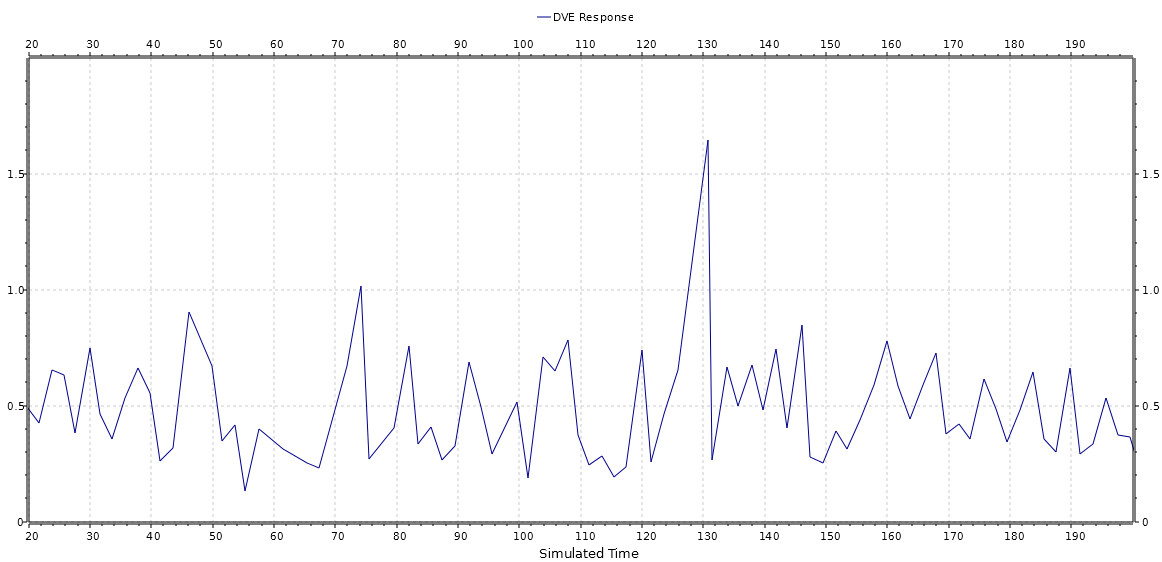
\includegraphics[scale=0.4]{response.jpeg}
\end{center}
\caption{Il \emph{Response Time} di un client.}
\label{response}
\end{figure}

\begin{figure}
\begin{center}
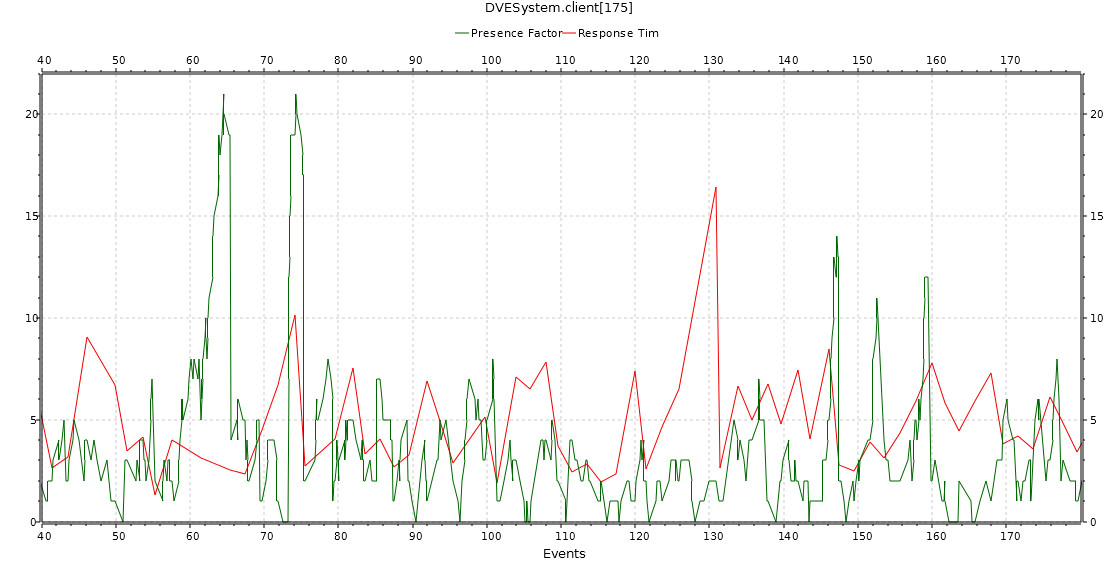
\includegraphics[scale=0.4]{responseVSpresence.jpeg}
\end{center}
\caption{Mancanza di correlazione tra \emph{Response Time} e
\emph{Presence Factor}.}
\label{responseVSPresence}
\end{figure}

\chapter{Conclusioni}\label{conclusioni}

%%\backmatter
%%% Bibliografia.
\cleardoublepage
\phantomsection
\addcontentsline{toc}{chapter}{Bibliografia}
\begin{thebibliography}{}

\bibitem{specifiche} Jacob Feldman\\
        \emph{JSR-331 Java Constraint Programming API SPECIFICATION} \\
        \footnotesize \texttt{http://openrules.com/downloads/jsr331/JSR331.Specification.v081.pdf} \normalsize

\bibitem{tesiAmadini} Roberto Amadini \\
	\emph{Studio e realizzazione in Java di domini e regole per la risoluzione di vincoli su interi e insiemi di interi} \\
	\footnotesize \texttt{http://www.cs.unipr.it/Informatica/Tesi/Roberto\_Amadini\_20111109.pdf} \normalsize

\bibitem{prolog} Luca Console, Evelina Lamma, Paola Mello, Michela Milano \\
	\emph{Programmazione Logica e Prolog} \\
	UTET Libreria srl, 1997.

\bibitem{intArt} Stuart Russell, Peter Norvig \\
	\emph{Intelligenza Artificiale \\ Un approccio moderno - Volume 1} \\
	Pearson Education Italia S.r.l., 2005.


\bibitem{artClp} A. Dovier, C. Piazza, E. Pontelli, G. Rossi \\
	\emph{Sets and constraint logic programming} \\
	ACM TOPLAS 2000; 22(5):861-931.

\bibitem{artJsetl} Gianfranco Rossi, Elio Panegai, Elisabetta Poleo \\
	\emph{JSetL: a Java library for supporting declarative programming in Java} \\
	Software Practice \& Experience 2007; 37:115-149.

\bibitem{jsetlMan} Gianfranco Rossi, Roberto Amadini \\
         \emph{JSetL User's Manual Version 2.3}\\
         "Quaderni del Dipartimento di Matematica", n. 507, Università di Parma, 24 Gennaio 2012.

\bibitem{jacop} JaCoP - Java Constraint Programming solver \\
	\texttt{http://jacop.osolpro.com/}

\bibitem{sitoJava} Java Platform, Standard Edition 6: API Specification \\
	\texttt{http://java.sun.com/javase/6/docs/api/}

\bibitem{jsetl} JSetL Home Page \\
	\texttt{http://cmt.math.unipr.it/jsetl.html}

\bibitem{blog}  Constraint Programming Standardization Blog\\
	\texttt{http://cpstandard.wordpress.com/}


\end{thebibliography}

\bibliographystyle{abbrv}
\bibliography{relazione}
\end{document}
